%%%%%%%%%%%%%%%%%%%%%%%%%%% asme2ej.tex %%%%%%%%%%%%%%%%%%%%%%%%%%%%%%%
% Template for producing ASME-format journal articles using LaTeX    %
% Written by   Harry H. Cheng, Professor and Director                %
%              Integration Engineering Laboratory                    %
%              Department of Mechanical and Aeronautical Engineering %
%              University of California                              %
%              Davis, CA 95616                                       %
%              Tel: (530) 752-5020 (office)                          %
%                   (530) 752-1028 (lab)                             %
%              Fax: (530) 752-4158                                   %
%              Email: hhcheng@ucdavis.edu                            %
%              WWW:   http://iel.ucdavis.edu/people/cheng.html       %
%              May 7, 1994                                           %
% Modified: February 16, 2001 by Harry H. Cheng                      %
% Modified: January  01, 2003 by Geoffrey R. Shiflett                %
% Butchered: October 15, 2014 by John Karasinski                     %
% Use at your own risk, send complaints to /dev/null                 %
%%%%%%%%%%%%%%%%%%%%%%%%%%%%%%%%%%%%%%%%%%%%%%%%%%%%%%%%%%%%%%%%%%%%%%

%%% use twocolumn and 10pt options with the asme2ej format
\documentclass[twocolumn,10pt]{asme2ej}

\usepackage{epsfig} %% for loading postscript figures
\usepackage{listings}
\usepackage{amsmath}
\usepackage{graphicx}
\usepackage{grffile}
\usepackage{pdfpages}
\usepackage{algpseudocode}

\title{Case Study \# 2: OpenFOAM–Lid-Driven Cavity Flow}

\author{John Karasinski
    \affiliation{
  Graduate Student Researcher\\
  Center for Human/Robotics/Vehicle Integration and Performance\\
  Department of Mechanical and Aerospace Engineering\\
  University of California\\
  Davis, California 95616\\
    Email: karasinski@ucdavis.edu
    }
}

\begin{document}
\maketitle

%%%%%%%%%%%%%%%%%%%%%%%%%%%%%%%%%%%%%%%%%%%%%%%%%%%%%%%%%%%%%%%%%%%%%%
\section{Problem Description}
The flow of an incompressible fluid induced in a square cavity by a moving upper boundary, or ``lid-driven'' cavity flow, is a classic validation case for Computational Fluid Dynamics (CFD) solvers. The top wall moves in the $x$-direction at a speed of 1 m/s while the other 3 are stationary. This case study involves performing numerical simulations of this flow problem for various flow regimes using an Open Source PDE solver: OpenFOAM \cite{jasak2007openfoam}. Initially, the flow will be assumed laminar and will be solved on a uniform mesh using the icoFoam solver for laminar, isothermal, incompressible flow. This problem is solved for a 129 x 129 uniform grid with Reynolds numbers of 100 and 1000, and a 257 x 257 uniform grid with Reynolds numbers of 5000 and 10000, and are analytically compared to previous results \cite{ghia1982high}.

%%%%%%%%%%%%%%%%%%%%%%%%%%%%%%%%%%%%%%%%%%%%%%%%%%%%%%%%%%%%%%%%%%%%%%
\section{Solver Setup}
The installation of OpenFOAM is a nontrivial process. While official online documentation lists installation instructions for choice Linux distributions, there is no official documentation for installing OpenFOAM on OS X. Fortunately, some users have documentated their installations and made the steps available online \cite{ctfm_1}.

OpenFOAM 2.3.0 can be built on OS X 10.9 fairly simply by making use of Homebrew (a free/open source software package management system that simplifies the installation of software on the OS X). Homebrew, when used alongside additional command lines tools such as curl and git, greatly simplifies the installation of OpenFOAM. Installation instructions are available in Appendix A. Before running these instructions, however, Paraview must first be install. Paraview has readibly avaialble precombiled binaries which can be installed in a normal fashion.

To confirm that OpenFOAM has been installed correctly, the guide recommends running the lid-driven cavity flow example which comes installed with OpenFOAM \cite{ctfm_1}. After the files are copied into a local directory, the example can be run via the following terminal commands:
\begin{lstlisting}[language=sh]
$ blockMesh
$ icoFoam
\end{lstlisting}
which should result in a large amount of text being outputted to the screen. The user can then run the \lstinline[language=sh]`paraFoam` command to view the resulting simulation data.

%%%%%%%%%%%%%%%%%%%%%%%%%%%%%%%%%%%%%%%%%%%%%%%%%%%%%%%%%%%%%%%%%%%%%%
\section{Numerical Solution}
Numerical solutions were found for the lid-driven cavity flow problem for a 129 x 129 uniform grid with Reynolds numbers of 100, and 1000, and a 257 x 257 grid with Reynolds numbers of 5000 and 10000. To do this, the OpenFOAM icoFoam example, `cavity' was used.

The initial mesh was set to be 129 x 129 grid points (by adjusting line 33 of the blockMeshDict file) and was generated with the \lstinline[language=sh]`blockMesh` command. To insure that the simulation runs to convergence (and given the quickness at which the simulation runs), the simulation end time is set to 30 seconds (line 26 of the controlDict file). Other default values were used, and the only values changed between runs were $Re$, the Reynolds number, and the step time, deltaT. This is done by adjusting $\nu$, the kinematic viscosity, which relates to the Reynolds number via:
\begin{equation}
Re = \frac{d|U|}{\nu},
\end{equation}
where $d = 0.1$m is the characteristic length, and $|U| = 1$ ms$^{-1}$ is the characteristic velocity. A Reynolds number of 100, for instance, can be achieved by setting $\nu = 0.001$m$^2$s$^{-1}$ (line 18 of the transportProperties file). For both of the 129 x 129 grid cases, a step time of 0.005 was used. For the 257 x 257 grid with a Reynolds number of 5000, a time step of 0.001 was used, while the simulation with a Reynolds number of 10000 required a time step of 0.0001. After generating the grid and adjusting other necessary parameters, the simulation can be run via the \lstinline[language=sh]`icoFoam` command. Once the simulation has finished running, the streamfunction can be generated with the \lstinline[language=sh]`streamFunction` command.

\begin{figure}[htb]
\begin{center}
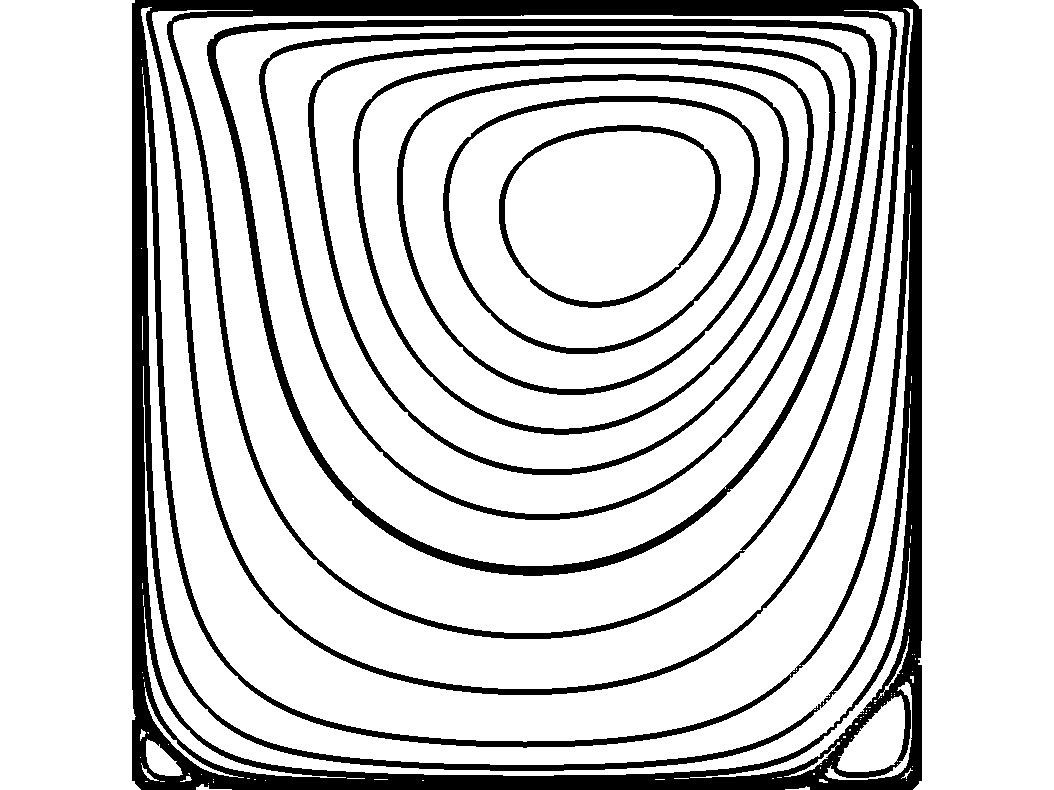
\includegraphics[width=0.5\textwidth]{figure/Re100.png}
\caption{$Re = 100$ at $t = 30$, Uniform Grid (129 x 129)}
\label{Re100}
\vspace{5mm} %5mm vertical space
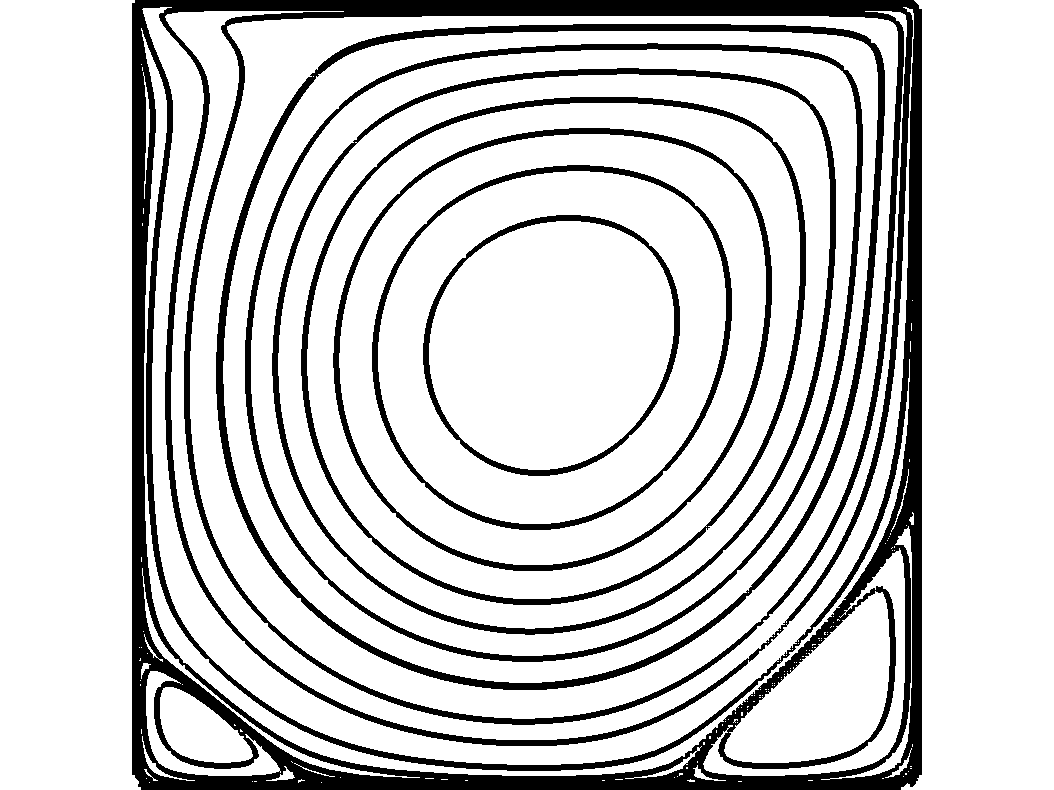
\includegraphics[width=0.5\textwidth]{figure/Re1000.png}
\caption{$Re = 1000$ at $t = 30$, Uniform Grid (129 x 129)}
\label{Re1000}
\vspace{5mm} %5mm vertical space
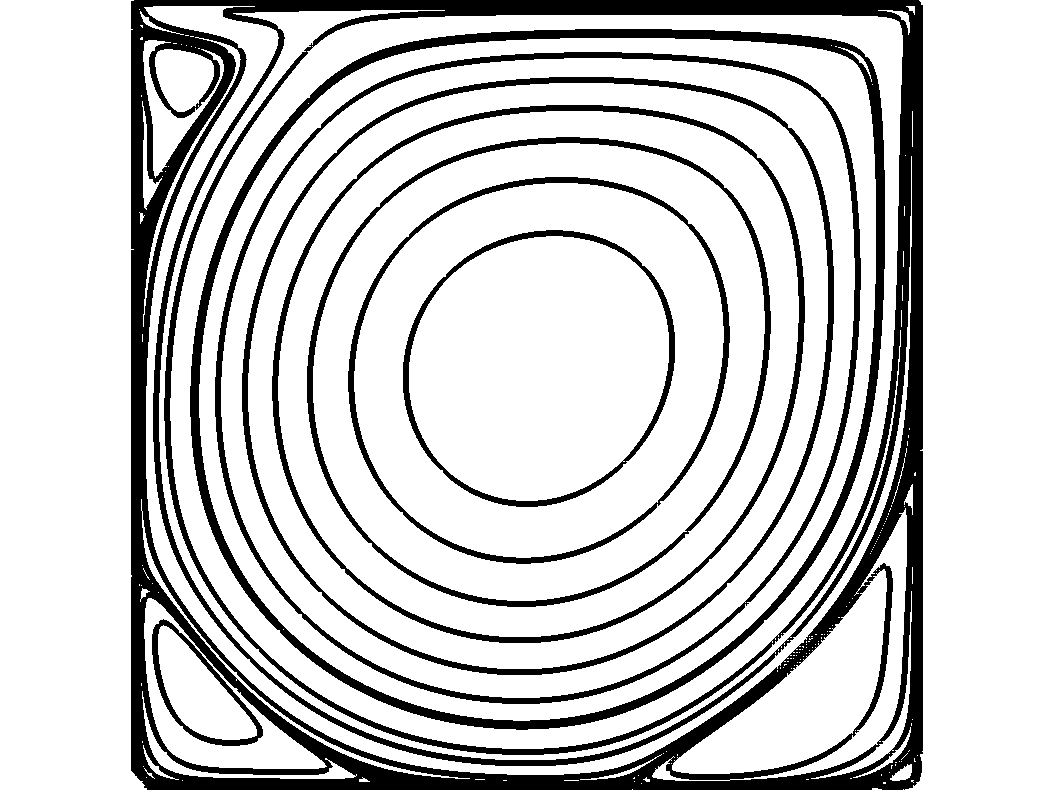
\includegraphics[width=0.5\textwidth]{figure/Re5000.png}
\caption{$Re = 5000$ at $t = 30$, Uniform Grid (257 x 257)}
\label{Re5000}
\end{center}
\end{figure}

\begin{figure}[htb]
\begin{center}
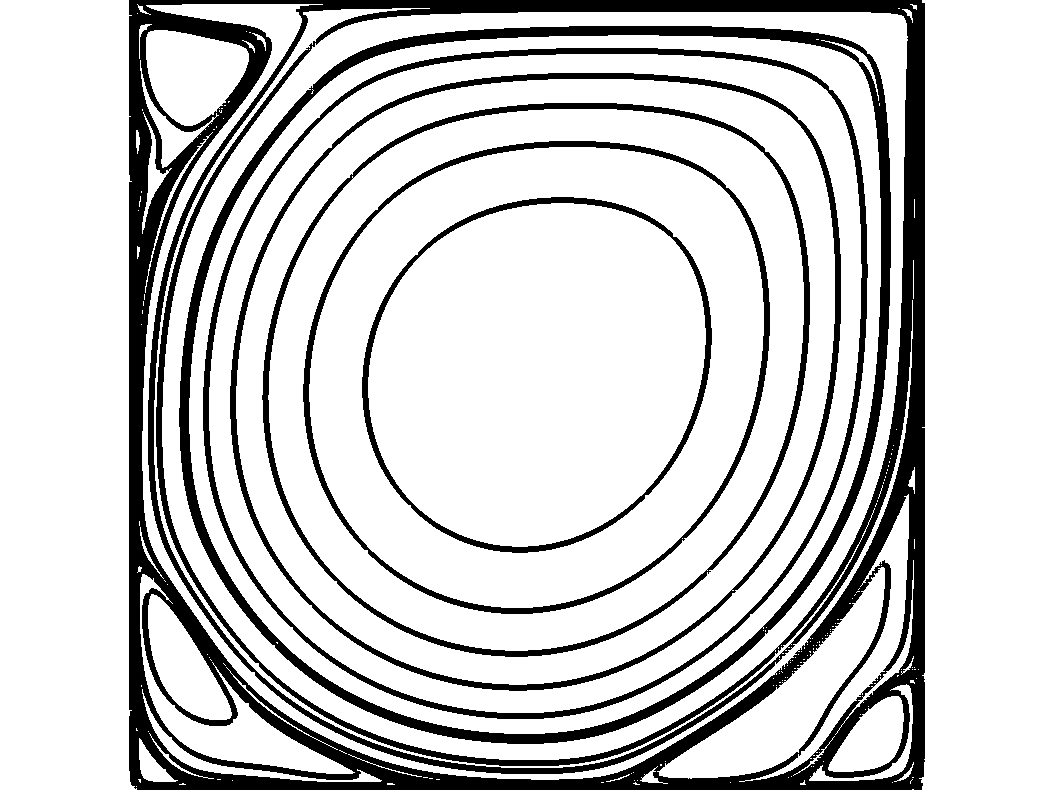
\includegraphics[width=0.5\textwidth]{figure/Re10000.png}
\caption{$Re = 10000$ at $t = 18.7$, Uniform Grid (257 x 257)}
\label{Re10000}
\vspace{5mm} %5mm vertical space
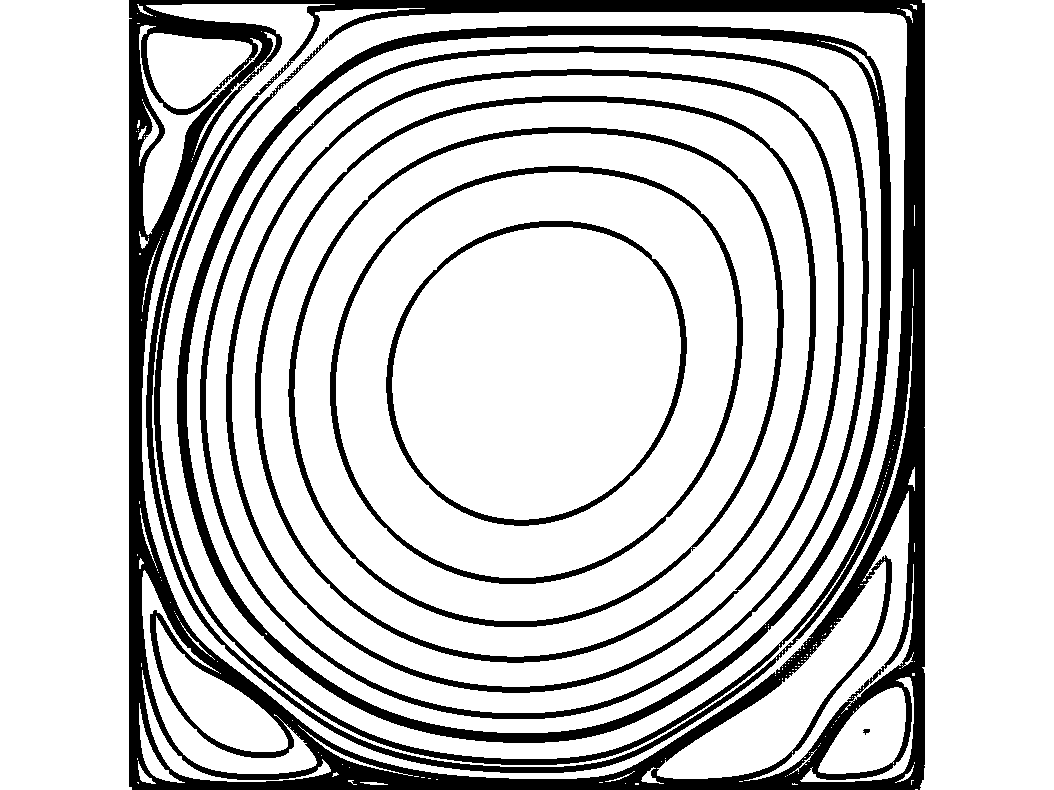
\includegraphics[width=0.5\textwidth]{figure/Re10000-fin.png}
\caption{$Re = 10000$ at $t = 30$, Uniform Grid (257 x 257)}
\label{Re10000-fin}
\end{center}
\end{figure}

%%%%%%%%%%%%%%%%%%%%%%%%%%%%%%%%%%%%%%%%%%%%%%%%%%%%%%%%%%%%%%%%%%%%%%
\section{Discussion and Conclusions}
Qualitative comparisons of streamlines to results previously published in the literature suggest a good match to the methods presented here for both the 129 x 129 and 257 x 257 uniform grids \cite{ghia1982high}.

The results from OpenFOAM for Reynolds numbers of 100, 1000, and 5000 match previous results quite well. The results from the Reynolds number of 100 show the two characteristic eddies reported in previous results, one in the bottom left (BL$_1$) and one in the bottom right (BR$_1$). Figure \ref{Re100} shows the streamlines for this case. Similarly, the results for the Reynolds number of 1000 show both eddies BL$_1$ and BR$_1$, and also hints at an additional eddie in the bottom right corner, BR$_2$. This case also shows the beginning of separation of flow from the upper left corner (see Figure \ref{Re1000}). Increasing both the grid size (to 257 x 257) and the Reynolds number to 5000 makes the BL$_2$ eddie more clear, as was the case in previous studies. Setting the Reynolds number to 5000 also leads to the formation of an additional eddie in the top left corner (TL$_1$), as can be seen in Figure \ref{Re5000}. These three cases show a steady laminar flow which compares well to previously published results.

The steady solution for $Re = 10000$, however, is no longer stable. This effect can be explained by a Hopf bifurcation which occurs around $Re = 8000$ and leads to some periodicity in the formation and dissipation of transient eddies \cite{bruneau20062d}. Careful selection of the output time can lead to results that look nearly identical to those published in the previous result \cite{ghia1982high}. In Figure \ref{Re10000} the six eddies in the literature, TL$_1$, BL$_1$, BL$_2$, BR$_1$, BR$_2$, and BR$_3$ can be seen, but these results are only transient. Choosing the final timestep (Figure \ref{Re10000-fin}), however, shows different results that can be explained by the loss of stability. Refining the mesh would allow for additional eddies to become apparent, and the transition between these periodic states would become more obvious.

%%%%%%%%%%%%%%%%%%%%%%%%%%%%%%%%%%%%%%%%%%%%%%%%%%%%%%%%%%%%%%%%%%%%%%
% \hfill \break
\bibliographystyle{asmems4}
\bibliography{asme2e}

%%%%%%%%%%%%%%%%%%%%%%%%%%%%%%%%%%%%%%%%%%%%%%%%%%%%%%%%%%%%%%%%%%%%%%
\clearpage
\onecolumn
\appendix
\section*{Appendix A: OpenFOAM 2.3.0 installation}

\begin{figure}[b]
\begin{center}
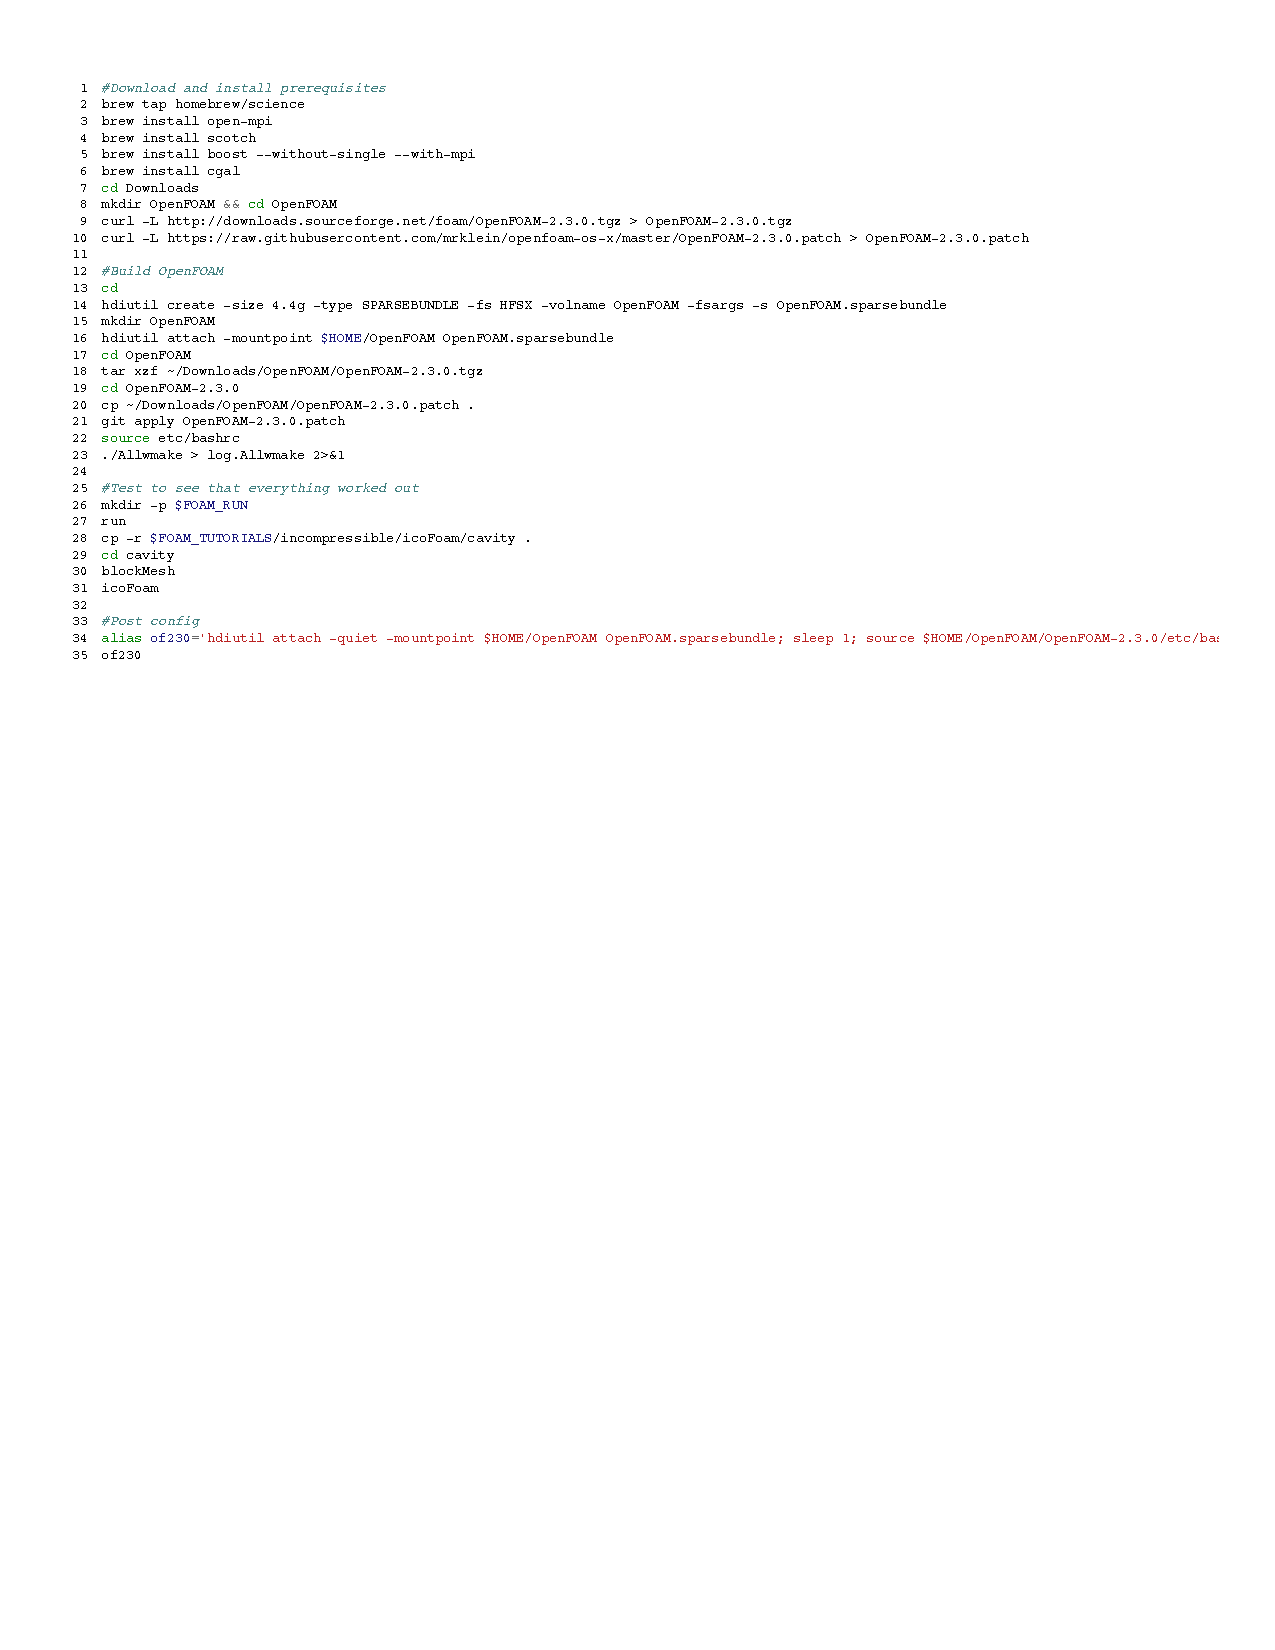
\includegraphics[page=1,width=0.93\textwidth]{of230_install.pdf}
\end{center}
\end{figure}

%%%%%%%%%%%%%%%%%%%%%%%%%%%%%%%%%%%%%%%%%%%%%%%%%%%%%%%%%%%%%%%%%%%%%%
\end{document}
